\begin{minipage}[t][\PosterRowHeightC][t]{\PosterColWidth}\vspace{0pt}
  \begin{PosterPanel}{\PosterRowHeightC}{7}{CO-DESIGN ALGORITHM}

    \noindent\begin{minipage}[t]{120mm}\vspace{0pt}
      \begin{tikzpicture}[x=1mm,y=1mm,font=\fontsize{19pt}{21pt}\selectfont,
        st/.style={draw=IASDarkGreen,fill=IASPaleGreen,line width=1pt,rounded corners=1.2mm,minimum height=15mm,text width=108mm,align=left,inner sep=1.2mm},
        ar/.style={-{Stealth[length=2.6mm]},line width=1.1pt,color=IASDarkGreen}]
        \node[st] (s1) at (0,0) {\textbf{1} open PLLs, keep grid: $G(s)$};
        \node[st] (s2) at (0,-19) {\textbf{2} diagnose: $\mathrm{eig}(Q)$, cycles $p_{ij}$};
        \node[st] (s3) at (0,-38) {\textbf{3} gain map or transport\\$\lambda\mapsto(k_p,k_I)$};
        \node[st] (s4) at (0,-57) {\textbf{4} predict: $\min\tfrac12|\delta|^2$\\s.t. $\mathrm{Re}\lambda_r+g_r\!\cdot\!\delta\le-\sigma$};
        \node[st,fill=IASPaleGold] (s5) at (0,-76) {\textbf{5} correct: exact spectrum,\\shrink step if worse};
        \node[st] (s6) at (0,-95) {\textbf{6} verify: roots + five events};
        \foreach \a/\b in {s1/s2,s2/s3,s3/s4,s4/s5,s5/s6}{\draw[ar] (\a) -- (\b);}
        \draw[ar,color=IASVermillion] (s5.east) -- ++(5,0) |- (s4.east);
      \end{tikzpicture}
      \vspace{4mm}
      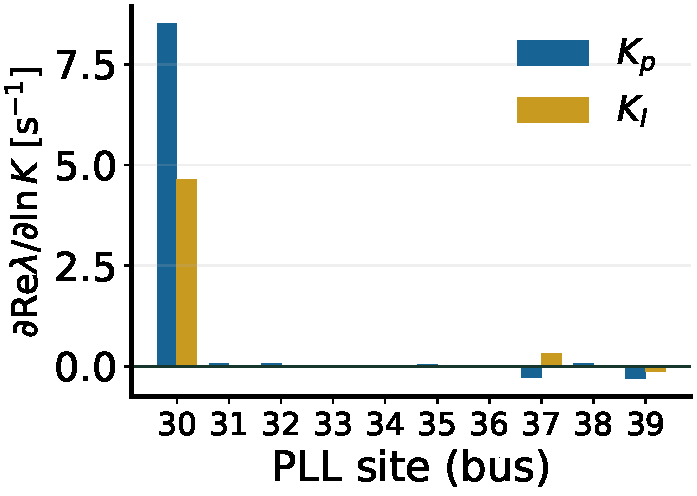
\includegraphics[width=118mm,height=84mm,keepaspectratio]{generated/figures/authority.pdf}\par
      {\fontsize{20pt}{23pt}\selectfont Leading 44 ms root: authority sits at site 30 (8.5\,s$^{-1}$ per $\ln K_p$), not at the cycle pair 35--36 ($\le0.05$).\par}
    \end{minipage}\hfill%
    \begin{minipage}[t]{146mm}\vspace{0pt}
      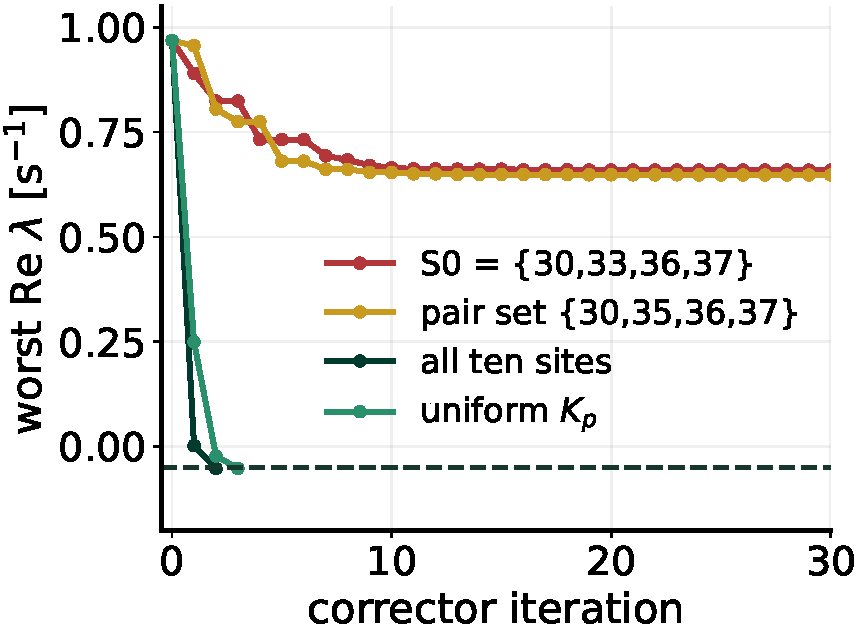
\includegraphics[width=146mm,height=108mm,keepaspectratio]{generated/figures/repair_curve.pdf}\par
      {\fontsize{20pt}{23pt}\selectfont Worst root per iteration, 44 ms.\par}
      \vspace{1mm}
      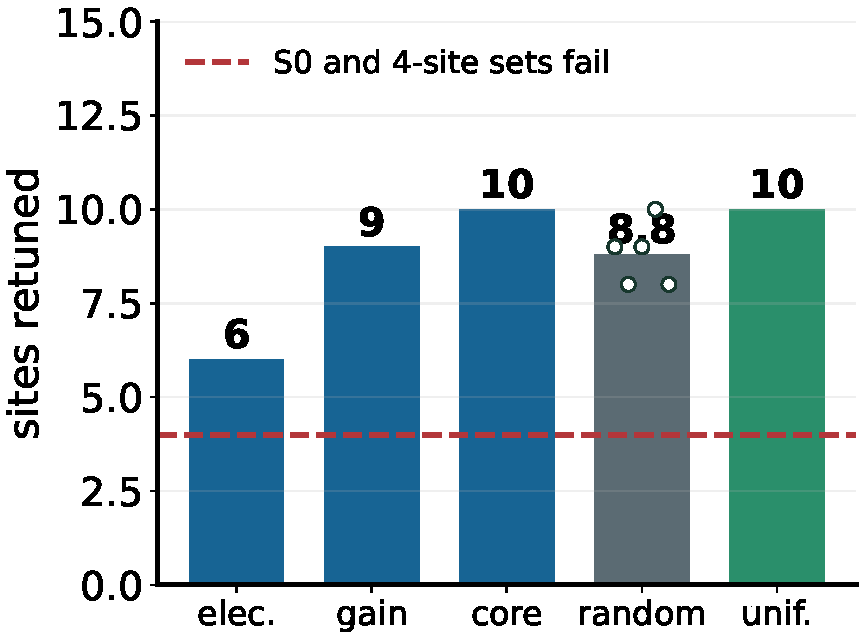
\includegraphics[width=146mm,height=108mm,keepaspectratio]{generated/figures/support_scan.pdf}\par
      {\fontsize{20pt}{23pt}\selectfont Sites retuned until the margin holds.\par}
    \end{minipage}\par
    \vspace{1mm}
    {\fontsize{22pt}{25pt}\selectfont \textbf{$S_0=\{30,33,36,37\}$ fails} ($K_I$, $K_p$, joint); so does every four-site set. One common $K_p$ cut of 14\,\% restores the margin.\par}

  \end{PosterPanel}
\end{minipage}%
